\documentclass{extbook}[14pt]
\usepackage{multicol, enumerate, enumitem, hyperref, color, soul, setspace, parskip, fancyhdr, amssymb, amsthm, amsmath, bbm, latexsym, units, mathtools}
\everymath{\displaystyle}
\usepackage[headsep=0.5cm,headheight=0cm, left=1 in,right= 1 in,top= 1 in,bottom= 1 in]{geometry}
\usepackage{dashrule}  % Package to use the command below to create lines between items
\newcommand{\litem}[1]{\item #1

\rule{\textwidth}{0.4pt}}
\pagestyle{fancy}
\lhead{}
\chead{Answer Key for Module6 Version B}
\rhead{}
\lfoot{9356-6875}
\cfoot{}
\rfoot{testing}
\begin{document}
\textbf{This key should allow you to understand why you choose the option you did (beyond just getting a question right or wrong). \href{https://xronos.clas.ufl.edu/mac1105spring2020/courseDescriptionAndMisc/Exams/LearningFromResults}{More instructions on how to use this key can be found here}.}

\textbf{If you have a suggestion to make the keys better, \href{https://forms.gle/CZkbZmPbC9XALEE88}{please fill out the short survey here}.}

\textit{Note: This key is auto-generated and may contain issues and/or errors. The keys are reviewed after each exam to ensure grading is done accurately. If there are issues (like duplicate options), they are noted in the offline gradebook. The keys are a work-in-progress to give students as many resources to improve as possible.}

\rule{\textwidth}{0.4pt}

\begin{enumerate}\litem{
Describe the end behavior of the polynomial below.
\[ f(x) = -9(x - 4)^{3}(x + 4)^{8}(x + 9)^{3}(x - 9)^{3} \]The solution is the graph below, which is option A.
\begin{center}
    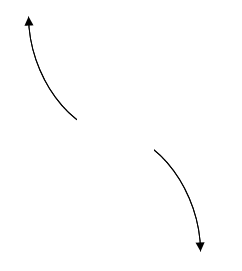
\includegraphics[width=0.3\textwidth]{../Figures/polyEndBehaviorAB.png}
\end{center}\begin{enumerate}[label=\Alph*.]
\begin{multicols}{2}
\item 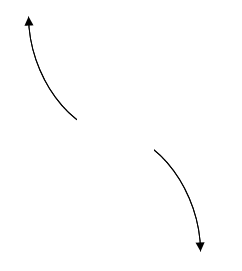
\includegraphics[width = 0.3\textwidth]{../Figures/polyEndBehaviorAB.png}
\item 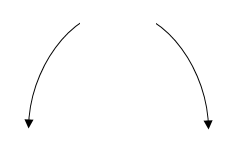
\includegraphics[width = 0.3\textwidth]{../Figures/polyEndBehaviorBB.png}
\item 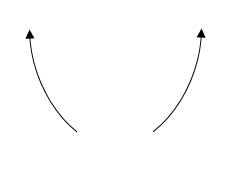
\includegraphics[width = 0.3\textwidth]{../Figures/polyEndBehaviorCB.png}
\item 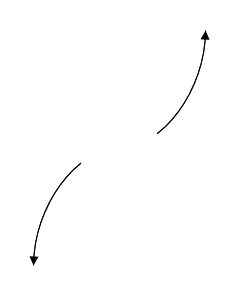
\includegraphics[width = 0.3\textwidth]{../Figures/polyEndBehaviorDB.png}
\end{multicols}\item None of the above.\end{enumerate}
\textbf{General Comment:} Remember that end behavior is determined by the leading coefficient AND whether the \textbf{sum} of the multiplicities is positive or negative.
}
\litem{
Which of the following equations \textit{could} be of the graph presented below?

\begin{center}
    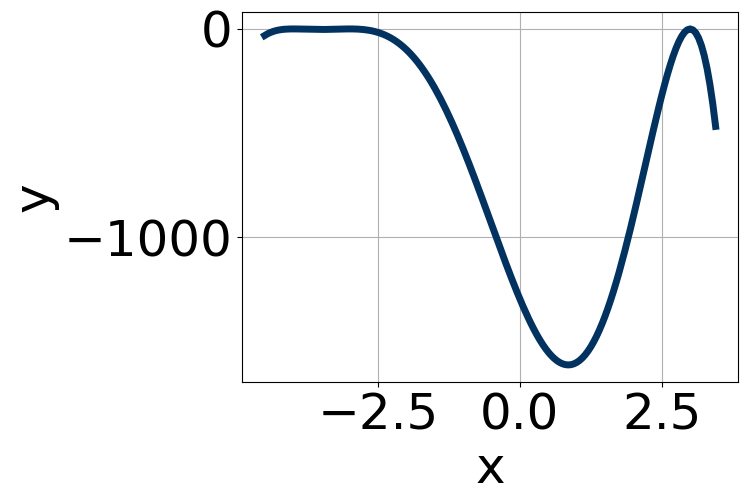
\includegraphics[width=0.5\textwidth]{../Figures/polyGraphToFunctionB.png}
\end{center}


The solution is \( 6(x + 1)^{11} (x - 3)^{11} (x - 1)^{9} \), which is option E.\begin{enumerate}[label=\Alph*.]
\item \( -14(x + 1)^{5} (x - 3)^{11} (x - 1)^{9} \)

This corresponds to the leading coefficient being the opposite value than it should be.
\item \( 20(x + 1)^{6} (x - 3)^{10} (x - 1)^{5} \)

The factors $-1$ and $3$ have have been odd power.
\item \( 12(x + 1)^{4} (x - 3)^{5} (x - 1)^{9} \)

The factor $-1$ should have been an odd power.
\item \( -11(x + 1)^{10} (x - 3)^{5} (x - 1)^{7} \)

The factor $(x + 1)$ should have an odd power and the leading coefficient should be the opposite sign.
\item \( 6(x + 1)^{11} (x - 3)^{11} (x - 1)^{9} \)

* This is the correct option.
\end{enumerate}

\textbf{General Comment:} General Comments: Draw the x-axis to determine which zeros are touching (and so have even multiplicity) or cross (and have odd multiplicity).
}
\litem{
Construct the lowest-degree polynomial given the zeros below. Then, choose the intervals that contain the coefficients of the polynomial in the form $ax^3+bx^2+cx+d$.
\[ \frac{3}{5}, -5, \text{ and } -7 \]The solution is \( 5x^{3} +57 x^{2} +139 x -105 \), which is option E.\begin{enumerate}[label=\Alph*.]
\item \( a \in [3, 17], b \in [-61, -55], c \in [131, 141], \text{ and } d \in [104, 111] \)

$5x^{3} -57 x^{2} +139 x + 105$, which corresponds to multiplying out $(5x + 3)(x -5)(x -7)$.
\item \( a \in [3, 17], b \in [62, 68], c \in [208, 220], \text{ and } d \in [104, 111] \)

$5x^{3} +63 x^{2} +211 x + 105$, which corresponds to multiplying out $(5x + 3)(x + 5)(x + 7)$.
\item \( a \in [3, 17], b \in [56, 59], c \in [131, 141], \text{ and } d \in [104, 111] \)

$5x^{3} +57 x^{2} +139 x + 105$, which corresponds to multiplying everything correctly except the constant term.
\item \( a \in [3, 17], b \in [4, 14], c \in [-173, -167], \text{ and } d \in [-106, -101] \)

$5x^{3} +13 x^{2} -169 x -105$, which corresponds to multiplying out $(5x + 3)(x -5)(x + 7)$.
\item \( a \in [3, 17], b \in [56, 59], c \in [131, 141], \text{ and } d \in [-106, -101] \)

* $5x^{3} +57 x^{2} +139 x -105$, which is the correct option.
\end{enumerate}

\textbf{General Comment:} To construct the lowest-degree polynomial, you want to multiply out $(5x -3)(x + 5)(x + 7)$
}
\litem{
Construct the lowest-degree polynomial given the zeros below. Then, choose the intervals that contain the coefficients of the polynomial in the form $x^3+bx^2+cx+d$.
\[ 4 + 3 i \text{ and } -4 \]The solution is \( x^{3} -4 x^{2} -7 x + 100 \), which is option D.\begin{enumerate}[label=\Alph*.]
\item \( b \in [0.1, 1.1], c \in [-0.68, 0.29], \text{ and } d \in [-17.9, -15.3] \)

$x^{3} + x^{2} -16$, which corresponds to multiplying out $(x -4)(x + 4)$.
\item \( b \in [3, 6.4], c \in [-7.36, -6.73], \text{ and } d \in [-101.4, -98.9] \)

$x^{3} +4 x^{2} -7 x -100$, which corresponds to multiplying out $(x-(4 + 3 i))(x-(4 - 3 i))(x -4)$.
\item \( b \in [0.1, 1.1], c \in [0.54, 2.17], \text{ and } d \in [-13.2, -10.4] \)

$x^{3} + x^{2} +x -12$, which corresponds to multiplying out $(x -3)(x + 4)$.
\item \( b \in [-5, -2.6], c \in [-7.36, -6.73], \text{ and } d \in [98.6, 102.8] \)

* $x^{3} -4 x^{2} -7 x + 100$, which is the correct option.
\item \( \text{None of the above.} \)

This corresponds to making an unanticipated error or not understanding how to use nonreal complex numbers to create the lowest-degree polynomial. If you chose this and are not sure what you did wrong, please contact the coordinator for help.
\end{enumerate}

\textbf{General Comment:} Remember that the conjugate of $a+bi$ is $a-bi$. Since these zeros always come in pairs, we need to multiply out $(x-(4 + 3 i))(x-(4 - 3 i))(x-(-4))$.
}
\litem{
Construct the lowest-degree polynomial given the zeros below. Then, choose the intervals that contain the coefficients of the polynomial in the form $ax^3+bx^2+cx+d$.
\[ \frac{-4}{3}, -2, \text{ and } \frac{3}{2} \]The solution is \( 6x^{3} +11 x^{2} -14 x -24 \), which is option C.\begin{enumerate}[label=\Alph*.]
\item \( a \in [6, 11], b \in [-7, -3], c \in [-23, -21], \text{ and } d \in [23, 25] \)

$6x^{3} -5 x^{2} -22 x + 24$, which corresponds to multiplying out $(3x -4)(x + 2)(2x -3)$.
\item \( a \in [6, 11], b \in [-15, -9], c \in [-14, -11], \text{ and } d \in [23, 25] \)

$6x^{3} -11 x^{2} -14 x + 24$, which corresponds to multiplying out $(3x -4)(x -2)(2x + 3)$.
\item \( a \in [6, 11], b \in [8, 16], c \in [-14, -11], \text{ and } d \in [-31, -20] \)

* $6x^{3} +11 x^{2} -14 x -24$, which is the correct option.
\item \( a \in [6, 11], b \in [-35, -27], c \in [46, 47], \text{ and } d \in [-31, -20] \)

$6x^{3} -29 x^{2} +46 x -24$, which corresponds to multiplying out $(3x -4)(x -2)(2x -3)$.
\item \( a \in [6, 11], b \in [8, 16], c \in [-14, -11], \text{ and } d \in [23, 25] \)

$6x^{3} +11 x^{2} -14 x + 24$, which corresponds to multiplying everything correctly except the constant term.
\end{enumerate}

\textbf{General Comment:} To construct the lowest-degree polynomial, you want to multiply out $(3x + 4)(x + 2)(2x -3)$
}
\litem{
Construct the lowest-degree polynomial given the zeros below. Then, choose the intervals that contain the coefficients of the polynomial in the form $x^3+bx^2+cx+d$.
\[ -5 + 4 i \text{ and } -3 \]The solution is \( x^{3} +13 x^{2} +71 x + 123 \), which is option A.\begin{enumerate}[label=\Alph*.]
\item \( b \in [12, 15], c \in [60, 72], \text{ and } d \in [122, 124] \)

* $x^{3} +13 x^{2} +71 x + 123$, which is the correct option.
\item \( b \in [-6, 3], c \in [-9, 0], \text{ and } d \in [-15, -4] \)

$x^{3} + x^{2} -x -12$, which corresponds to multiplying out $(x -4)(x + 3)$.
\item \( b \in [-18, -8], c \in [60, 72], \text{ and } d \in [-124, -121] \)

$x^{3} -13 x^{2} +71 x -123$, which corresponds to multiplying out $(x-(-5 + 4 i))(x-(-5 - 4 i))(x -3)$.
\item \( b \in [-6, 3], c \in [6, 14], \text{ and } d \in [6, 19] \)

$x^{3} + x^{2} +8 x + 15$, which corresponds to multiplying out $(x + 5)(x + 3)$.
\item \( \text{None of the above.} \)

This corresponds to making an unanticipated error or not understanding how to use nonreal complex numbers to create the lowest-degree polynomial. If you chose this and are not sure what you did wrong, please contact the coordinator for help.
\end{enumerate}

\textbf{General Comment:} Remember that the conjugate of $a+bi$ is $a-bi$. Since these zeros always come in pairs, we need to multiply out $(x-(-5 + 4 i))(x-(-5 - 4 i))(x-(-3))$.
}
\litem{
Describe the end behavior of the polynomial below.
\[ f(x) = -8(x - 2)^{4}(x + 2)^{7}(x + 8)^{2}(x - 8)^{3} \]The solution is the graph below, which is option B.
\begin{center}
    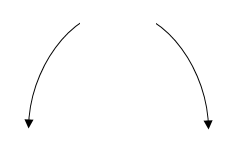
\includegraphics[width=0.3\textwidth]{../Figures/polyEndBehaviorCopyBB.png}
\end{center}\begin{enumerate}[label=\Alph*.]
\begin{multicols}{2}
\item 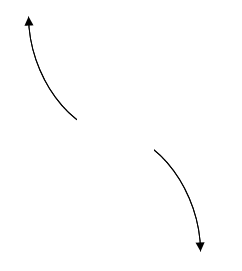
\includegraphics[width = 0.3\textwidth]{../Figures/polyEndBehaviorCopyAB.png}
\item 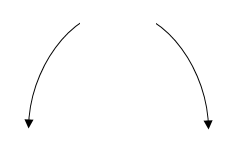
\includegraphics[width = 0.3\textwidth]{../Figures/polyEndBehaviorCopyBB.png}
\item 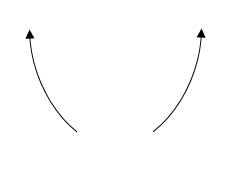
\includegraphics[width = 0.3\textwidth]{../Figures/polyEndBehaviorCopyCB.png}
\item 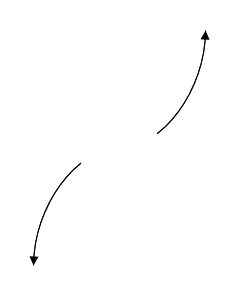
\includegraphics[width = 0.3\textwidth]{../Figures/polyEndBehaviorCopyDB.png}
\end{multicols}\item None of the above.\end{enumerate}
\textbf{General Comment:} Remember that end behavior is determined by the leading coefficient AND whether the \textbf{sum} of the multiplicities is positive or negative.
}
\litem{
Describe the zero behavior of the zero $x = -8$ of the polynomial below.
\[ f(x) = 6(x - 2)^{4}(x + 2)^{3}(x + 8)^{6}(x - 8)^{3} \]The solution is the graph below, which is option C.
\begin{center}
    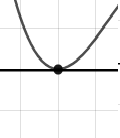
\includegraphics[width=0.3\textwidth]{../Figures/polyZeroBehaviorCB.png}
\end{center}\begin{enumerate}[label=\Alph*.]
\begin{multicols}{2}
\item 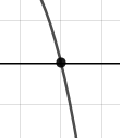
\includegraphics[width = 0.3\textwidth]{../Figures/polyZeroBehaviorAB.png}
\item 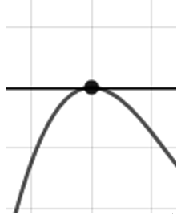
\includegraphics[width = 0.3\textwidth]{../Figures/polyZeroBehaviorBB.png}
\item 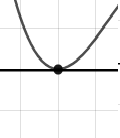
\includegraphics[width = 0.3\textwidth]{../Figures/polyZeroBehaviorCB.png}
\item 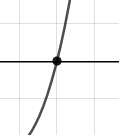
\includegraphics[width = 0.3\textwidth]{../Figures/polyZeroBehaviorDB.png}
\end{multicols}\item None of the above.\end{enumerate}
\textbf{General Comment:} You will need to sketch the entire graph, then zoom in on the zero the question asks about.
}
\litem{
Describe the zero behavior of the zero $x = -9$ of the polynomial below.
\[ f(x) = 3(x + 9)^{8}(x - 9)^{9}(x - 4)^{3}(x + 4)^{7} \]The solution is the graph below, which is option B.
\begin{center}
    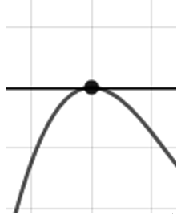
\includegraphics[width=0.3\textwidth]{../Figures/polyZeroBehaviorCopyBB.png}
\end{center}\begin{enumerate}[label=\Alph*.]
\begin{multicols}{2}
\item 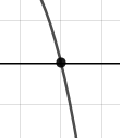
\includegraphics[width = 0.3\textwidth]{../Figures/polyZeroBehaviorCopyAB.png}
\item 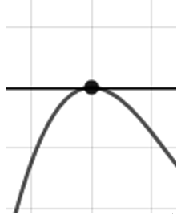
\includegraphics[width = 0.3\textwidth]{../Figures/polyZeroBehaviorCopyBB.png}
\item 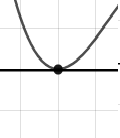
\includegraphics[width = 0.3\textwidth]{../Figures/polyZeroBehaviorCopyCB.png}
\item 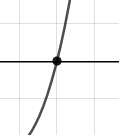
\includegraphics[width = 0.3\textwidth]{../Figures/polyZeroBehaviorCopyDB.png}
\end{multicols}\item None of the above.\end{enumerate}
\textbf{General Comment:} You will need to sketch the entire graph, then zoom in on the zero the question asks about.
}
\litem{
Which of the following equations \textit{could} be of the graph presented below?

\begin{center}
    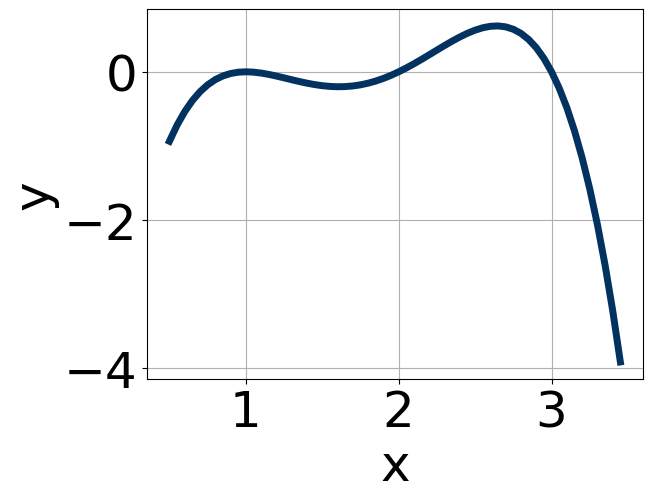
\includegraphics[width=0.5\textwidth]{../Figures/polyGraphToFunctionCopyB.png}
\end{center}


The solution is \( 13(x - 1)^{11} (x + 1)^{11} (x - 2)^{5} \), which is option A.\begin{enumerate}[label=\Alph*.]
\item \( 13(x - 1)^{11} (x + 1)^{11} (x - 2)^{5} \)

* This is the correct option.
\item \( 14(x - 1)^{4} (x + 1)^{9} (x - 2)^{9} \)

The factor $1$ should have been an odd power.
\item \( -10(x - 1)^{5} (x + 1)^{9} (x - 2)^{11} \)

This corresponds to the leading coefficient being the opposite value than it should be.
\item \( -19(x - 1)^{10} (x + 1)^{9} (x - 2)^{9} \)

The factor $(x - 1)$ should have an odd power and the leading coefficient should be the opposite sign.
\item \( 9(x - 1)^{4} (x + 1)^{8} (x - 2)^{11} \)

The factors $1$ and $-1$ have have been odd power.
\end{enumerate}

\textbf{General Comment:} General Comments: Draw the x-axis to determine which zeros are touching (and so have even multiplicity) or cross (and have odd multiplicity).
}
\end{enumerate}

\end{document}